%--------------------------------------------------------
% BEER PONG RULES: SETUP SECTION
%--------------------------------------------------------
\section{Setup}\label{sec:SETUP}
	\subsection{Cup Formation}\label{ssec:CupFormation}
		\begin{enumerate}[label=(\roman*)]
            \item \label{sssec:CF,solocups} Each player's rack is to be made up of 10 red 18 US-fluid-ounce solo cups.
                See \hyperref[fig:solocup]{Figure \ref{fig:solocup}} for the regulation cup specifications. 
            \item \label{sssec:CF,triangle} The starting rack is a tight equilateral triangle with the base towards the player's table edge and the tip towards the opponent. 
            \item \label{sssec:CF,position} The rack's back edge is to be at least two finger widths from the edge but no more than 4 and centred from side to side. 
            \item \label{sssec:CF,kissing} Solo Cup rims must be ``kissing". There should be minimal spaces in between the cups but not so close as to lean, tilt, or overlap onto their neighbouring cups. 
        \end{enumerate}
        \begin{figure}[H]% Shows a single rack setup
            \centering
            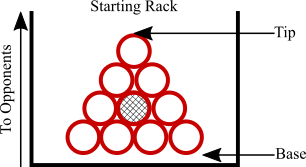
\includegraphics[width=0.3\textwidth]{startingrack.png}
            \caption{Diagram of a full 10 rack of cups, centred on the table. The arrow points towards the opponent's rack. The hashed middle cup is the bitch cup (see \ref{ssec:BitchCup}).}
            \label{fig:therack}
        \end{figure}
	\subsection{Cup Content}\label{ssec:CupContent}
        \begin{enumerate}[label=(\roman*)]
            \item \label{sssec:CC,filling} Cups are to be filled to a minimum that stops the moving and sliding when a ball is sunk into the cup. 
            \item \label{sssec:CC,w_vs_l} The physical content of the cup is either water or liquor.
                \begin{enumerate}[label=(\alph*), leftmargin=2cm]
                    \item Water Cups: Water is put into the cups following \hyperref[sssec:CC,filling]{Section \ref{sssec:CC,filling}} regulations
                    \item Drink Cups: Drinks are put into the solo cups following \hyperref[sssec:CC,filling]{Section \ref{sssec:CC,filling}} regulations and budget costs...
                \end{enumerate} 
            \item \label{sssec:CC,rinse} A cup of water will be provided to the players to rinse the balls off when playing with beer. This is for sanitary reasons. 
        \end{enumerate}        
    \subsection{The Balls}\label{ssec:Balls}
        \begin{enumerate}[label=(\roman*)]
            \item \label{sssec:Balls,num} The game is played with 2, 1.57in or 40mm diameter, Ping Pong Balls. See \hyperref[fig:solocup]{Figure \ref{fig:solocup}}.
            \item \label{sssec:Balls,dents} The balls must have no dents. 
            \item \label{sssec:Balls,bounce} The balls must be checked to have the same elasticity (bounce). 
            \item \label{sssec:Balls,texture} The texture of the balls must be consistent between the two; to the player's standards. This is for consistency of throwing. 
        \end{enumerate}    
	\subsection{The Cup}\label{ssec:Cup}
        \begin{enumerate}[label=(\roman*)]
            \item \label{sssec:Cup,dim} The solo cups are to be red, 18US-fluid-ounces and have the dimensions as seen in \hyperref[fig:solocup]{Figure \ref{fig:solocup}}. 
            \item \label{sssec:Cup,broken} Cups should not be used if broken or cracked in any way. Change this cup out. 
            \item \label{ssec:Cup,rinsing} Cups should be rinsed before a game in both water and drink versions before play. Cups can get quite gross. 
        \end{enumerate}
        \begin{figure}[H]
            \centering
            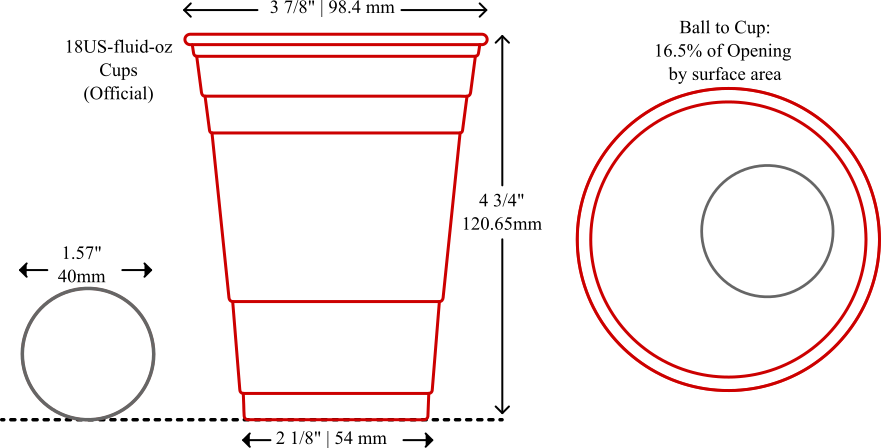
\includegraphics[width=0.9\textwidth]{dimensions.png}
            \caption{Dimensions of a regulation 18oz Solo Cup and Regulation ping pong ball.}
            \label{fig:solocup}
        \end{figure}
	\subsection{Teams}\label{ssec:Teams}
		\begin{enumerate}[label=(\roman*)]
            \item \label{sssec:teams,options} There are two options to play beer pong: single or doubles. 
                \begin{enumerate}[label=(\alph*), leftmargin=2cm]% Singles vs doubles
                    \item \textbf{Singles:} Beer pong can played as singles where for each rack there is one player.
                        This player will throw two balls each go (see Appendix \ref{app:A}).
                        The two balls (first and second throw) are independent of rules such as ``on-fire" and ``bounce".
                    \item \textbf{Doubles:}	This is a variation still played with two ping pong balls where each member of the team now throws a single ball.
                        Again, each ball is considered independent for rules such as ``on-fire" and ``bounce" but this time it is by player and not throw order.
                \end{enumerate} 
            \item \label{sssec:teams,choosing} There are no set rules for how teams are formed. Figure it out bud. 
        \end{enumerate}
	\subsection{The Table}\label{ssec:Table}
        \begin{enumerate}[label=(\roman*)]
            \item \label{sssec:Table,sides} The table is split into two sides down the midline (see \hyperref[fig:table]{Figure \ref{fig:table}}).
			    The opponents take opposite sides of the table. 
			    From the midpoint on the table in the direction the player is considered ``their side". 
            \item \label{sssec:Table,switch} If multiple games in a row are being played by the same players, they must switch sides every game. 
            \item \label{sssec:Table,length} The table must be at least 5ft long. 
        \end{enumerate}
        \begin{figure}[H]
            \centering
            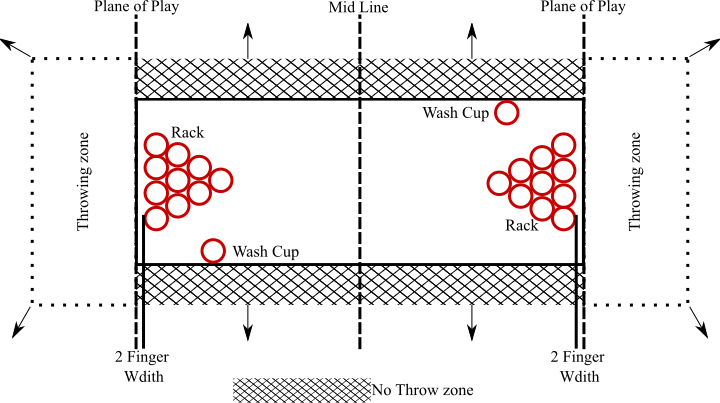
\includegraphics[width=\textwidth]{table.png}
            \caption{The table viewed from the top showing two racks, accepted throwing zones, the midpoint, and the 2 fingers from the edge that the rack has to be.}
            \label{fig:table}
        \end{figure}